\documentclass[twocolumn,oneside]{amsart}
\usepackage[utf8]{inputenc}
\usepackage[a4paper]{geometry}
\usepackage{tikz}
\usetikzlibrary{shapes,arrows}
\usepackage{pgfplots}
\usepackage{listings}
\usepackage{float}
\usepackage{subfig}
\pgfplotsset{compat=1.8}
\usepgfplotslibrary{statistics}
\newcommand{\fitnessplot}[1]{
\begin{tikzpicture}
\begin{axis}
[
axis x line=bottom,
axis y line=left,
width=\textwidth / 2,
xmax=20,
xmin=0,
ymax=1.05,
ymin=0.21,
axis y discontinuity=crunch,
extra y ticks={1.0},
extra y tick style={
    grid=major
},
scaled x ticks={real:0.2},
xtick scale label code/.code={},
boxplot/draw direction=y,
xlabel=Generation,
ylabel=Fitness,
]
#1
\end{axis}
\end{tikzpicture}
}


\usepackage{listings}
\usepackage{color}

\definecolor{mygreen}{rgb}{0,0.6,0}
\definecolor{mygray}{rgb}{0.5,0.5,0.5}
\definecolor{mymauve}{rgb}{0.58,0,0.82}

\lstset{ %
    backgroundcolor=\color{white},   % choose the background color; you must add \usepackage{color} or \usepackage{xcolor}
    basicstyle=\footnotesize,        % the size of the fonts that are used for the code
    breakatwhitespace=false,         % sets if automatic breaks should only happen at whitespace
    captionpos=b,                    % sets the caption-position to bottom
    commentstyle=\color{mygreen},    % comment style
    deletekeywords={...},            % if you want to delete keywords from the given language
    escapeinside={\%*}{*)},          % if you want to add LaTeX within your code
        extendedchars=true,              % lets you use non-ASCII characters; for 8-bits encodings only, does not work with UTF-8
        frame=single,                    % adds a frame around the code
        keepspaces=true,                 % keeps spaces in text, useful for keeping indentation of code (possibly needs columns=flexible)
        keywordstyle=\color{blue},       % keyword style
        language=Octave,                 % the language of the code
        morekeywords={*,...},            % if you want to add more keywords to the set
        numbers=none,                    % where to put the line-numbers; possible values are (none, left, right)
        numbersep=5pt,                   % how far the line-numbers are from the code
        numberstyle=\tiny\color{mygray}, % the style that is used for the line-numbers
        rulecolor=\color{black},         % if not set, the frame-color may be changed on line-breaks within not-black text (e.g. comments (green here))
        showspaces=false,                % show spaces everywhere adding particular underscores; it overrides 'showstringspaces'
        showstringspaces=false,          % underline spaces within strings only
        showtabs=false,                  % show tabs within strings adding particular underscores
        stepnumber=2,                    % the step between two line-numbers. If it's 1, each line will be numbered
        stringstyle=\color{mymauve},     % string literal style
        tabsize=2,                       % sets default tabsize to 2 spaces
        title=\lstname                   % show the filename of files included with \lstinputlisting; also try caption instead of title
    }

\title{Homework Module: \textbf{Programming the Basics of an Evolutionary Algorithm(EA)}}

\author{Sigve Sebastian Farstad}

\begin{document}

\newgeometry{top=3cm,bottom=3cm}
\maketitle

\section{Introduction}

This report presents a solution to Homework Module: Programming the Basics of an Evolutionary Algorithm(EA), IT3708, spring 2014, NTNU.
The assignment is to implement all of the basic components of an evolutionary algorithm, and use them to solve the One-Max problem.

\section{The Evolutionary Algorithm Implementation}

The evolutionary algorithm solver presented in this solution is implemented as a modular python library.
A generic solver function solves arbitrary problems supplied by the user of the library.

\begin{figure}
\tikzstyle{action} = [rectangle, draw,
        text width=5em, text centered, minimum height=3em]
\tikzstyle{line} = [draw, -latex']
\begin{tikzpicture}[node distance = 1.6cm, auto]
    \tikzstyle{every node}=[font=\small]
    % Place nodes
    \node [action] (init) {Generate initial child population};
    \node [action, below of=init] (phen) {Phenotype development};
    \node [action, right of=phen, node distance=3cm] (fitn) {Fitness evaluation};
    \node [action, below of=fitn] (asel) {Adult selection};
    \node [action, below of=asel] (psel) {Parent selection};
    \node [action, left of=psel, node distance=3cm] (cros) {Crossover};
    \node [action, above of=cros] (muta) {Mutation};
    \node [action, above of=fitn] (goal) {Accept solution};
    % Draw edges
    \path [line] (init) -- (phen);
    \path [line] (phen) -- (fitn);
    \path [line] (fitn) -- (asel);
    \path [line] (asel) -- (psel);
    \path [line] (psel) -- (cros);
    \path [line] (cros) -- (muta);
    \path [line] (muta) -- (phen);
    \path [line] (fitn) -- (goal);
\end{tikzpicture}
\caption{An abstract overview of the algorithm flow.}
\label{figure:flow}
\end{figure}

The flow of the evolutionary algorithm is identical to the one proposed in section 1 of \textit{EA Appendices}\footnote{K. Downing, EA Appendices, January 19, 2014}
and is illustrated in figure \ref{figure:flow}.

Each step in the algorithm can be implemented using different strategies.
Different strategies have different success rates for different problems, so it is important to choose a good strategy for a given problem.
Because of this, the solver library implements multiple different strategies for each step of the algorithm.
The different implemented strategies are elaborated upon in the following sections.

\subsection{Adult Selection}
Adult selection is the process of selecting individuals from the children pool and the adult pool to form the adult pool of the next generation.
As suggested in \textit{EA Appendices}, the solver implements three different strategies for adult selection: full generation replacement, over-production, and generation mixing.

\subsubsection{Full Generational Replacement}
Full generational replacement is an adult selection strategy where the adult population of generation $ n $ consists of the entire child population of generation $ n - 1 $.
It requires that the child and adult populations are equally large.

\subsubsection{Over-production}
Over-production is an adult selection strategy where the adult population of generation $ n $ consists of a true subset of the child population of generation $ n - 1 $.
The subset may be selected using many different methods.
Weighting the subset selection by fitness is a popular choice.
The implementation in the solver presented in this report uses unweighted random selection, as it is easier to implement.

Over-production requires that the child population is larger than the adult population.

\subsubsection{Generational Mixing}
Generational mixing is an adult selection strategy similar to over-production, except that the selected subset is a subset of both the child and adult populations from the previous generation, rather than just the child generation.
The same considerations for subset selection apply for generational mixing.
The implementation in the solver presented in this report uses unweighted random selection here, too.

Generational mixing does not impose any restrictions on population sizes.

\subsection{Parent Selection}
Parent selection is the process of selecting adults for combination in the crossover stage.
Parent selection strategies must take care to select fit individuals while at the same time allowing for the variance that allows the algorithm to avoid getting stuck at local maxima.
The presented solver implements five different parent selection strategies: fitness-proportionate selection, sigma scaling selection, tournament selection, rank selection, and random selection.

\subsubsection{Fitness-Proportionate Selection}
Fitness-proportionate selection is a selection scheme where an individual is selected at random, with the probability of being chosen equal to $ \frac{f(i)}{F} $, where $ f(i) $ is the fitness of an individual, and $ F $ is the total fitness of the population.

\subsubsection{Sigma Scaling Selection}
Sigma-scaling selection is similar to fitness-proportionate scaling, but the probability of a given individual being chosen is scaled by the fitness variance of the population, as in equation 3 of \textit{EA Appendices}.

\subsubsection{Tournament Selection}

Tournament selection is a selection scheme where a predefined $ k < | population | $ number of individuals are selected for participation in a tournament.
Of these competing individuals, the one with the greatest fitness score gets selected.
Some tournament selection implementations use a variant of fitness proportionate scaling to select the winner individual from the tournament participants, but that is not the case in the presented solver.
This is because always selecting the best individual amongst the tournament participants guarantees that the $ k - 1 $ worst individuals in a population will not get selected.

\subsubsection{Rank Selection}

Rank selection is a selection scheme similar to fitness-proportionate selection, only the probability of selection is defined as in equation \ref{equation:rank-selection}.

\begin{equation}\label{equation:rank-selection}
P_{sel} = 2 \times
\frac{rank(i)}
{| population | \times (| population | + 1)}
\end{equation}

\subsubsection{Random Selection}
Random selection is a selection scheme that simply selects an individual at random.
It is not a good selection scheme for an EA, but is included in the selection suite for benchmarking purposes.

\subsection{Crossover}
Crossover is a method for combining the genome of two individuals to create a new individual based on the originals.
The evolutionary algorithm implementation made for this assignment offers two different crossover strategies: split and per-component.

\subsubsection{Split Crossover}
Split crossover is a crossover scheme where a child's left part of its genome string comes from the first parent, and the right part of its genome string comes from the second parent.
The split point defining where the left part of a genome ends and the right part of a genome begins is chosen at random for each crossover.

\subsubsection{Per-component Crossover}
Per-component crossover is a crossover scheme where each component of a child's genome has an equal chance of coming from either the first or the second parent.


\subsection{Mutation}
Mutation is a method from introducing more variance into the population.
The presented solver randomly mutates individuals as they are entered into the child pool.
The mutation schemes in the presented solver can be supplied by the user as a part of a problem description, as good mutation schemes are highly problem-dependent.

\subsection{Modularity of the code}
The code is quite modular and reusable.
It is implemented as a generic library designed with extensibility in mind.
New phenotypes, genotypes, genetic operators and selection mechanisms may be developed and dropped in as replacements for existing functionality.
In regular use cases, the user needs only supply a fitness function, and configure which mechanisms shall be used.
Listing \ref{listing:configure} shows how easy configuration can be.
Listing \ref{listing:run} shows how to run the solver.

\begin{lstlisting}[frame=single,language=Python,caption={The One-Max problem being configured to be solved with tournament selection.},label={listing:configure}]
from ea.parent_selection
    import tournament_selection
...

class OneMax():
    ...
    parent_selection = \
        tournament_selection(k=8)
    ...
\end{lstlisting}

\begin{lstlisting}[frame=single,language=Python,caption={The solver solving the One-Max problem.},label={listing:run}]
from ea.solve import solve
...

ea.solve(OneMax())

\end{lstlisting}
\label{listing:run}

\section{The One-Max Problem}

The One-Max problem is a simple problem popularly chosen as a demonstration problem for testing evolutionary algorithm implementations.
It has no other real-world applications.
The problem is: what is the binary string of length $ n $ that contains the largest number of Ones?
The problem is trivial, but is good for basic evolutionary algorithm testing because of its transparency and simplicity.

\subsection{Genotype and Phenotype Representation}

A single genotype is represented as a binary vector of length $ n $.
Because of the simplicity of the program, the phenotype is identical.

\subsection{Fitness Evaluation}

The fitness function $ f_{\textsc{OneMax}}(g) $ of a genotype $ g $ is defined as equation \ref{equation:fitness}, where $ g_i $ is the $ i $\textsuperscript{th} bit of the genome $ g $.

\begin{equation}\label{equation:fitness}
f_{\textsc{OneMax}}(g) = \sum_{i=1}^{n} g_i
\end{equation}


\section{Performance analysis}

\subsection{Finding a population size}

Part of the assignment is to find an approximate minimal population size that consistently solves One-Max in less than 100 generations while using full generational adult replacement and fitness-proportionate parent selection.
The population size of 150 was empirically chosen.

\subsection{Crossover and mutation evaluation}

In order to measure the effect of crossover and mutation parameters, the solver was run with different parameters while adult selection was fixed to full generational replacement and parent selection was fixed to fitness-proportionate parent selection.
For each configuration tested, the solver was run 100 times, logging the number of generations until a solution was found for each run.
Results of the evaluation can be found represented as a box plot in figure \ref{figure:crossover-mutation}.

The results clearly show that it is important to keep the mutation rate low enough to allow for enough exploitation.
The results also seem to favor higher crossover rates.
The configuration $ P_{mutation} = 0.001, P_{crossover} = 1 $ is chosen as the best configuration for further analysis of other components in the system.
An illustration of an example run of a One-Max problem of size 40 being solved can be seen in \ref{figure:single-run}.

\subsection{Comparison of Parent Selection Mechanisms}

With the same parameters and strategies as in the previous section, the efficiency of the different available parent selection mechanisms was measured.
Again, each configuration was run 100 times.
The results can be seen in figure \ref{figure:selection-comparison}.
Random selection was also measured, but no test runs ever produced an acceptable solution, and is therefore not plotted in figure \ref{figure:selection-comparison}.

The results show that, of the different selection configurations tested, tournament selection with $ k = 8 $ gives the best results.

\subsection{Problem variations}

The One-Max problem is a special case of the more general problem of finding a specific known bit string in a known search space.
Changing the target bit string in the One-Max problem is not expected to change the difficulty of the problem, but it does require a modification to the fitness function.
To test this claim, the solver was tested on Known-Bitstring-Search, a problem similar to One-Max except that it tries to find a random bitstring rather than the bitstring composed of only $ 1 $.
Figure \ref{figure:problem-variation} shows convergence of Known-Bitstring-Search as solved by the presented solver compared to One-Max.

\begin{figure}[H]
\fitnessplot{
% generation 0
\addplot+[
boxplot prepared={
median=0.5625,
upper quartile=0.600625,
lower quartile=0.525625,
upper whisker=0.70140625,
lower whisker=0.36
},
] coordinates {};
% generation 5
\addplot+[
boxplot prepared={
median=0.58140625,
upper quartile=0.64,
lower quartile=0.54390625,
upper whisker=0.7225,
lower whisker=0.455625
},
] coordinates {};
% generation 10
\addplot+[
boxplot prepared={
median=0.62015625,
upper quartile=0.6551171875,
lower quartile=0.5625,
upper whisker=0.765625,
lower whisker=0.49
},
] coordinates {};
% generation 15
\addplot+[
boxplot prepared={
median=0.66015625,
upper quartile=0.70140625,
lower quartile=0.62015625,
upper whisker=0.78765625,
lower whisker=0.50765625
},
] coordinates {};
% generation 20
\addplot+[
boxplot prepared={
median=0.680625,
upper quartile=0.7385546875,
lower quartile=0.64,
upper whisker=0.87890625,
lower whisker=0.54390625
},
] coordinates {};
% generation 25
\addplot+[
boxplot prepared={
median=0.70140625,
upper quartile=0.74390625,
lower quartile=0.66015625,
upper whisker=0.92640625,
lower whisker=0.50765625
},
] coordinates {};
% generation 30
\addplot+[
boxplot prepared={
median=0.70140625,
upper quartile=0.74390625,
lower quartile=0.66015625,
upper whisker=0.855625,
lower whisker=0.5625
},
] coordinates {};
% generation 35
\addplot+[
boxplot prepared={
median=0.7225,
upper quartile=0.765625,
lower quartile=0.680625,
upper whisker=0.855625,
lower whisker=0.58140625
},
] coordinates {};
% generation 40
\addplot+[
boxplot prepared={
median=0.74390625,
upper quartile=0.81,
lower quartile=0.7225,
upper whisker=0.87890625,
lower whisker=0.62015625
},
] coordinates {};
% generation 45
\addplot+[
boxplot prepared={
median=0.765625,
upper quartile=0.81,
lower quartile=0.7225,
upper whisker=0.9025,
lower whisker=0.64
},
] coordinates {};
% generation 50
\addplot+[
boxplot prepared={
median=0.78765625,
upper quartile=0.83265625,
lower quartile=0.765625,
upper whisker=0.9025,
lower whisker=0.66015625
},
] coordinates {};
% generation 55
\addplot+[
boxplot prepared={
median=0.81,
upper quartile=0.83265625,
lower quartile=0.765625,
upper whisker=0.9025,
lower whisker=0.680625
},
] coordinates {};
% generation 60
\addplot+[
boxplot prepared={
median=0.81,
upper quartile=0.83265625,
lower quartile=0.78765625,
upper whisker=0.9025,
lower whisker=0.680625
},
] coordinates {};
% generation 65
\addplot+[
boxplot prepared={
median=0.83265625,
upper quartile=0.855625,
lower quartile=0.78765625,
upper whisker=0.92640625,
lower whisker=0.70140625
},
] coordinates {};
% generation 70
\addplot+[
boxplot prepared={
median=0.83265625,
upper quartile=0.8730859375,
lower quartile=0.78765625,
upper whisker=0.950625,
lower whisker=0.70140625
},
] coordinates {};
% generation 71
\addplot+[
boxplot prepared={
median=0.83265625,
upper quartile=0.884112563993,
lower quartile=0.781562436007,
upper whisker=1.0,
lower whisker=0.70140625
},
] coordinates {};
}

\caption{A single run of the solver solving a OneMax problem of size 40 using full generational adult selection, fitness-proportionate parent selection, per component crossover ($ p = 1 $), per genome component mutation ($ p = 0.001 $), and a population size of 150.}
\label{figure:single-run}
\end{figure}

\onecolumn

\begin{figure}
\subfloat[Solution efficiency of the algorithm for different configurations of probability of mutation $ P_m $, and probability of crossover $ P_c $. The graph truncates at 1000 generations.]{%
\label{figure:crossover-mutation}
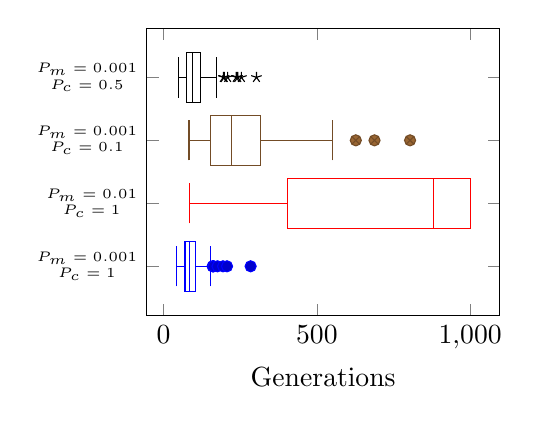
\begin{tikzpicture}
\begin{axis}
[
width=\textwidth/2,
ytick={1, 2, 3 , 4},
yticklabels={
    {$ P_{m} = 0.001 $ \\ $ P_{c} = 1 $},
    {$ P_{m} = 0.01 $ \\ $ P_{c} = 1 $},
    {$ P_{m} = 0.001 $ \\ $ P_{c} = 0.1 $},
    {$ P_{m} = 0.001 $ \\ $ P_{c} = 0.5 $}
},
yticklabel style={align=center,font=\tiny},
xlabel=Generations
]
\addplot+[boxplot]
table[row sep=\\, y index=0] {
% pgmutate 0.001, pgcrossover 1, fgr, fps, pop 150
data\\
62\\ 207\\ 90\\ 56\\ 116\\ 194\\ 98\\ 86\\ 58\\ 66\\
81\\ 65\\ 77\\ 74\\ 89\\ 66\\ 83\\ 99\\ 90\\ 84\\ 72\\
63\\ 101\\ 97\\ 151\\ 114\\ 90\\ 163\\ 106\\ 70\\ 65\\
107\\ 73\\ 69\\ 133\\ 88\\ 105\\ 94\\ 176\\ 160\\ 68\\
100\\ 73\\ 79\\ 67\\ 76\\ 140\\ 64\\ 86\\ 41\\ 100\\
91\\ 58\\ 70\\ 61\\ 90\\ 60\\ 91\\ 66\\ 105\\ 89\\ 104\\
73\\ 75\\ 94\\ 76\\ 71\\ 115\\ 83\\ 81\\ 78\\ 125\\
141\\ 73\\ 69\\ 86\\ 121\\ 103\\ 84\\ 65\\ 59\\ 45\\
73\\ 107\\ 81\\ 58\\ 162\\ 86\\ 115\\ 80\\ 113\\ 94\\
57\\ 105\\ 152\\ 75\\ 284\\ 76\\ 77\\ 68\\
};

\addplot+[boxplot]
table[row sep=\\, y index=0] {
% pgmutate 0.01, pgcrossover 1, fgr, fps, pop 150
data\\
483\\ 1000\\ 578\\ 597\\ 1000\\ 1000\\ 497\\ 796\\ 760\\ 800\\ 1000\\ 1000\\ 1000\\ 1000\\ 1000\\ 1000\\ 1000\\ 855\\ 96\\ 361\\ 162\\ 1000\\ 334\\ 1000\\ 888\\ 1000\\ 924\\ 110\\ 153\\ 985\\ 1000\\ 1000\\ 610\\ 425\\ 1000\\ 1000\\ 1000\\ 691\\ 160\\ 592\\ 464\\ 1000\\ 241\\ 811\\ 1000\\ 1000\\ 1000\\ 1000\\ 336\\ 954\\ 469\\ 1000\\ 1000\\ 1000\\ 699\\ 1000\\ 133\\ 277\\ 321\\ 278\\ 1000\\ 1000\\ 189\\ 829\\ 393\\ 881\\ 1000\\ 207\\ 505\\ 1000\\ 422\\ 1000\\ 1000\\ 85\\ 1000\\ 499\\ 1000\\ 729\\ 428\\ 1000\\ 1000\\ 216\\ 1000\\ 341\\ 253\\ 177\\ 1000\\ 1000\\ 1000\\ 188\\ 888\\ 1000\\ 525\\ 842\\ 386\\ 1000\\ 403\\ 1000\\ 881\\ 117\\
};
\addplot+[boxplot]
table[row sep=\\, y index=0] {
% pgmutate 0.001, pgcrossover 0.1, fgr, fps, pop 150
data\\
83\\ 487\\ 110\\ 487\\ 118\\ 171\\ 154\\ 287\\ 95\\ 224\\ 97\\ 124\\ 379\\ 348\\ 251\\ 164\\ 276\\ 298\\ 378\\ 214\\ 472\\ 270\\ 117\\ 358\\ 117\\ 523\\ 146\\ 371\\ 134\\ 142\\ 157\\ 208\\ 305\\ 127\\ 286\\ 187\\ 417\\ 688\\ 458\\ 274\\ 223\\ 188\\ 158\\ 228\\ 337\\ 218\\ 145\\ 234\\ 235\\ 179\\ 206\\ 359\\ 212\\ 627\\ 137\\ 200\\ 149\\ 271\\ 108\\ 168\\ 274\\ 316\\ 145\\ 504\\ 396\\ 283\\ 256\\ 550\\ 345\\ 271\\ 187\\ 299\\ 198\\ 376\\ 146\\ 188\\ 122\\ 256\\ 126\\ 254\\ 248\\ 231\\ 276\\ 218\\ 138\\ 155\\ 335\\ 212\\ 211\\ 356\\ 222\\ 174\\ 351\\ 147\\ 189\\ 152\\ 804\\ 129\\ 502\\ 125\\
};
\addplot+[boxplot]
table[row sep=\\, y index=0] {
% pgmutate 0.001, pgcrossover 0.5, fgr, fps, pop 150
data\\
117\\ 86\\ 242\\ 140\\ 105\\ 112\\ 88\\ 66\\ 209\\ 63\\ 130\\ 136\\ 84\\ 95\\ 96\\ 84\\ 50\\ 254\\ 73\\ 169\\ 121\\ 303\\ 90\\ 95\\ 84\\ 195\\ 56\\ 61\\ 104\\ 66\\ 157\\ 84\\ 102\\ 109\\ 69\\ 69\\ 94\\ 58\\ 139\\ 118\\ 81\\ 97\\ 103\\ 104\\ 145\\ 65\\ 78\\ 93\\ 67\\ 83\\ 96\\ 167\\ 148\\ 90\\ 68\\ 198\\ 95\\ 62\\ 84\\ 75\\ 112\\ 127\\ 95\\ 99\\ 81\\ 172\\ 109\\ 100\\ 76\\ 59\\ 89\\ 55\\ 75\\ 119\\ 57\\ 160\\ 87\\ 90\\ 94\\ 116\\ 122\\ 135\\ 120\\ 88\\ 98\\ 104\\ 121\\ 237\\ 60\\ 111\\ 75\\ 172\\ 95\\ 65\\ 72\\ 167\\ 89\\ 88\\ 70\\ 69\\
};
\end{axis}
\end{tikzpicture}
%\caption{Solution efficiency of the algorithm for different configurations of probability of mutation $ P_m $, and probability of crossover $ P_c $, measured in number of generations until solution acceptance over 100 runs.}
%\label{figure:crossover-mutation}
}
\subfloat[Comparison of different selection mechanisms.]{%
\label{figure:selection-comparison}
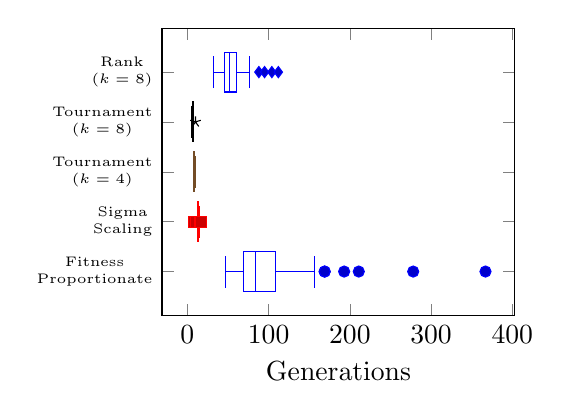
\begin{tikzpicture}
\begin{axis}
[
width=\textwidth/2,
ytick={1,2,3,4,5,6},
yticklabels={
    Fitness\\Proportionate,
    Sigma\\Scaling,
    Tournament\\($ k = 4 $),
    Tournament\\($ k = 8 $),
    Rank\\($ k = 8 $),
},
yticklabel style={align=center,font=\tiny},
xlabel=Generations
]
\addplot+[boxplot]
table[row sep=\\, y index=0] {
% pgmutate 0.001, pgcrossover 1, fgr, gps, pop 150
data\\
90\\ 69\\ 125\\ 119\\ 68\\ 90\\ 96\\ 127\\ 68\\ 119\\ 96\\ 169\\ 123\\ 78\\ 193\\ 61\\ 126\\ 54\\ 99\\ 50\\ 106\\ 64\\ 86\\ 119\\ 80\\ 52\\ 93\\ 123\\ 66\\ 81\\ 82\\ 64\\ 63\\ 84\\ 60\\ 149\\ 95\\ 86\\ 79\\ 87\\ 72\\ 150\\ 108\\ 106\\ 145\\ 103\\ 104\\ 116\\ 70\\ 79\\ 74\\ 103\\ 157\\ 89\\ 64\\ 76\\ 86\\ 78\\ 278\\ 72\\ 72\\ 169\\ 66\\ 88\\ 69\\ 106\\ 75\\ 80\\ 130\\ 83\\ 65\\ 76\\ 63\\ 60\\ 58\\ 52\\ 136\\ 102\\ 92\\ 77\\ 367\\ 117\\ 73\\ 122\\ 77\\ 77\\ 83\\ 66\\ 62\\ 80\\ 93\\ 115\\ 112\\ 69\\ 67\\ 76\\ 108\\ 211\\ 47\\ 88\\
};
\addplot+[boxplot]
table[row sep=\\, y index=0] {
% pgmutate 0.001, pgcrossover 1, fgr, sss, pop 150
data\\
14\\ 16\\ 14\\ 14\\ 11\\ 14\\ 13\\ 16\\ 15\\ 12\\ 14\\ 14\\ 13\\ 14\\ 13\\ 14\\ 15\\ 15\\ 14\\ 14\\ 13\\ 13\\ 13\\ 14\\ 13\\ 12\\ 14\\ 13\\ 14\\ 15\\ 14\\ 13\\ 14\\ 14\\ 11\\ 14\\ 15\\ 15\\ 14\\ 14\\ 13\\ 13\\ 14\\ 15\\ 12\\ 12\\ 13\\ 15\\ 16\\ 12\\ 13\\ 14\\ 13\\ 8\\ 11\\ 14\\ 13\\ 15\\ 12\\ 16\\ 11\\ 14\\ 15\\ 12\\ 13\\ 15\\ 11\\ 15\\ 14\\ 15\\ 14\\ 16\\ 13\\ 14\\ 13\\ 17\\ 14\\ 15\\ 14\\ 16\\ 12\\ 13\\ 13\\ 13\\ 14\\ 14\\ 13\\ 15\\ 13\\ 13\\ 14\\ 15\\ 14\\ 14\\ 14\\ 14\\ 14\\ 13\\ 14\\ 13\\
};
\addplot+[boxplot]
table[row sep=\\, y index=0] {
% pgmutate 0.001, pgcrossover 1, fgr, tsk4, pop 150
data\\
7\\ 8\\ 8\\ 9\\ 8\\ 9\\ 8\\ 8\\ 8\\ 8\\ 8\\ 8\\ 8\\ 9\\ 8\\ 7\\ 7\\ 8\\ 8\\ 8\\ 8\\ 9\\ 7\\ 8\\ 8\\ 9\\ 9\\ 8\\ 9\\ 9\\ 8\\ 9\\ 9\\ 9\\ 8\\ 9\\ 9\\ 9\\ 8\\ 8\\ 8\\ 9\\ 9\\ 8\\ 9\\ 7\\ 9\\ 9\\ 9\\ 9\\ 10\\ 9\\ 9\\ 9\\ 7\\ 9\\ 7\\ 7\\ 10\\ 9\\ 9\\ 8\\ 9\\ 8\\ 8\\ 8\\ 9\\ 9\\ 9\\ 7\\ 8\\ 9\\ 8\\ 9\\ 7\\ 9\\ 7\\ 8\\ 9\\ 7\\ 9\\ 9\\ 8\\ 9\\ 9\\ 10\\ 8\\ 8\\ 8\\ 8\\ 9\\ 9\\ 8\\ 10\\ 8\\ 8\\ 9\\ 9\\ 9\\ 8\\
};
\addplot+[boxplot]
table[row sep=\\, y index=0] {
% pgmutate 0.001, pgcrossover 1, fgr, tsk8, pop 150
data\\
7\\ 6\\ 6\\ 6\\ 7\\ 7\\ 5\\ 7\\ 7\\ 7\\ 8\\ 6\\ 6\\ 7\\ 7\\ 5\\ 7\\ 6\\ 7\\ 6\\ 7\\ 7\\ 7\\ 7\\ 7\\ 7\\ 7\\ 7\\ 7\\ 7\\ 7\\ 7\\ 7\\ 7\\ 7\\ 6\\ 7\\ 6\\ 6\\ 10\\ 7\\ 6\\ 6\\ 7\\ 6\\ 6\\ 7\\ 6\\ 7\\ 6\\ 7\\ 6\\ 7\\ 5\\ 6\\ 7\\ 7\\ 6\\ 6\\ 7\\ 7\\ 6\\ 7\\ 7\\ 7\\ 8\\ 7\\ 7\\ 7\\ 6\\ 7\\ 7\\ 7\\ 6\\ 8\\ 6\\ 7\\ 8\\ 7\\ 6\\ 7\\ 7\\ 7\\ 7\\ 6\\ 6\\ 7\\ 6\\ 7\\ 6\\ 7\\ 7\\ 6\\ 7\\ 7\\ 8\\ 6\\ 7\\ 6\\ 6\\
};
\addplot+[boxplot]
table[row sep=\\, y index=0] {
% pgmutate 0.001, pgcrossover 1, fgr, ranks, pop 150
data\\
56\\ 42\\ 51\\ 55\\ 43\\ 59\\ 36\\ 63\\ 32\\ 40\\ 53\\ 62\\ 57\\ 68\\ 46\\ 57\\ 54\\ 55\\ 61\\ 59\\ 54\\ 55\\ 63\\ 69\\ 32\\ 41\\ 49\\ 53\\ 57\\ 69\\ 73\\ 42\\ 112\\ 59\\ 61\\ 51\\ 58\\ 40\\ 49\\ 36\\ 42\\ 48\\ 46\\ 45\\ 61\\ 55\\ 46\\ 65\\ 49\\ 57\\ 52\\ 51\\ 58\\ 55\\ 43\\ 62\\ 64\\ 48\\ 50\\ 60\\ 50\\ 46\\ 43\\ 104\\ 43\\ 77\\ 49\\ 47\\ 51\\ 62\\ 43\\ 57\\ 41\\ 62\\ 62\\ 51\\ 75\\ 62\\ 57\\ 51\\ 37\\ 41\\ 62\\ 88\\ 37\\ 46\\ 40\\ 50\\ 53\\ 95\\ 59\\ 47\\ 44\\ 46\\ 47\\ 62\\ 40\\ 60\\ 37\\ 48\\
};
\end{axis}
\end{tikzpicture}
}
\qquad
\subfloat[Comparison of different selection mechanisms (zoom).]{%
\label{figure:selection-comparison}
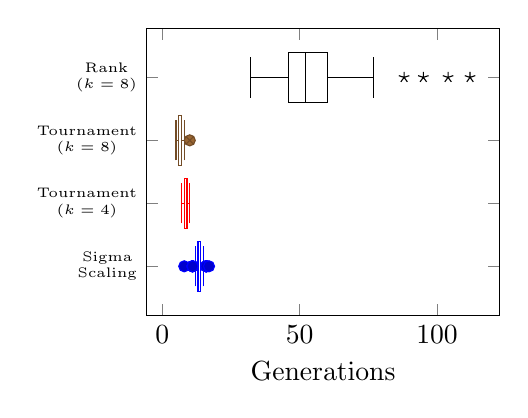
\begin{tikzpicture}
\begin{axis}
[
width=\textwidth/2,
ytick={1,2,3,4},
yticklabels={
    Sigma\\Scaling,
    Tournament\\($ k = 4 $),
    Tournament\\($ k = 8 $),
    Rank\\($ k = 8 $),
},
yticklabel style={align=center,font=\tiny},
xlabel=Generations
]
\addplot+[boxplot]
table[row sep=\\, y index=0] {
% pgmutate 0.001, pgcrossover 1, fgr, sss, pop 150
data\\
14\\ 16\\ 14\\ 14\\ 11\\ 14\\ 13\\ 16\\ 15\\ 12\\ 14\\ 14\\ 13\\ 14\\ 13\\ 14\\ 15\\ 15\\ 14\\ 14\\ 13\\ 13\\ 13\\ 14\\ 13\\ 12\\ 14\\ 13\\ 14\\ 15\\ 14\\ 13\\ 14\\ 14\\ 11\\ 14\\ 15\\ 15\\ 14\\ 14\\ 13\\ 13\\ 14\\ 15\\ 12\\ 12\\ 13\\ 15\\ 16\\ 12\\ 13\\ 14\\ 13\\ 8\\ 11\\ 14\\ 13\\ 15\\ 12\\ 16\\ 11\\ 14\\ 15\\ 12\\ 13\\ 15\\ 11\\ 15\\ 14\\ 15\\ 14\\ 16\\ 13\\ 14\\ 13\\ 17\\ 14\\ 15\\ 14\\ 16\\ 12\\ 13\\ 13\\ 13\\ 14\\ 14\\ 13\\ 15\\ 13\\ 13\\ 14\\ 15\\ 14\\ 14\\ 14\\ 14\\ 14\\ 13\\ 14\\ 13\\
};
\addplot+[boxplot]
table[row sep=\\, y index=0] {
% pgmutate 0.001, pgcrossover 1, fgr, tsk4, pop 150
data\\
7\\ 8\\ 8\\ 9\\ 8\\ 9\\ 8\\ 8\\ 8\\ 8\\ 8\\ 8\\ 8\\ 9\\ 8\\ 7\\ 7\\ 8\\ 8\\ 8\\ 8\\ 9\\ 7\\ 8\\ 8\\ 9\\ 9\\ 8\\ 9\\ 9\\ 8\\ 9\\ 9\\ 9\\ 8\\ 9\\ 9\\ 9\\ 8\\ 8\\ 8\\ 9\\ 9\\ 8\\ 9\\ 7\\ 9\\ 9\\ 9\\ 9\\ 10\\ 9\\ 9\\ 9\\ 7\\ 9\\ 7\\ 7\\ 10\\ 9\\ 9\\ 8\\ 9\\ 8\\ 8\\ 8\\ 9\\ 9\\ 9\\ 7\\ 8\\ 9\\ 8\\ 9\\ 7\\ 9\\ 7\\ 8\\ 9\\ 7\\ 9\\ 9\\ 8\\ 9\\ 9\\ 10\\ 8\\ 8\\ 8\\ 8\\ 9\\ 9\\ 8\\ 10\\ 8\\ 8\\ 9\\ 9\\ 9\\ 8\\
};
\addplot+[boxplot]
table[row sep=\\, y index=0] {
% pgmutate 0.001, pgcrossover 1, fgr, tsk8, pop 150
data\\
7\\ 6\\ 6\\ 6\\ 7\\ 7\\ 5\\ 7\\ 7\\ 7\\ 8\\ 6\\ 6\\ 7\\ 7\\ 5\\ 7\\ 6\\ 7\\ 6\\ 7\\ 7\\ 7\\ 7\\ 7\\ 7\\ 7\\ 7\\ 7\\ 7\\ 7\\ 7\\ 7\\ 7\\ 7\\ 6\\ 7\\ 6\\ 6\\ 10\\ 7\\ 6\\ 6\\ 7\\ 6\\ 6\\ 7\\ 6\\ 7\\ 6\\ 7\\ 6\\ 7\\ 5\\ 6\\ 7\\ 7\\ 6\\ 6\\ 7\\ 7\\ 6\\ 7\\ 7\\ 7\\ 8\\ 7\\ 7\\ 7\\ 6\\ 7\\ 7\\ 7\\ 6\\ 8\\ 6\\ 7\\ 8\\ 7\\ 6\\ 7\\ 7\\ 7\\ 7\\ 6\\ 6\\ 7\\ 6\\ 7\\ 6\\ 7\\ 7\\ 6\\ 7\\ 7\\ 8\\ 6\\ 7\\ 6\\ 6\\
};
\addplot+[boxplot]
table[row sep=\\, y index=0] {
% pgmutate 0.001, pgcrossover 1, fgr, ranks, pop 150
data\\
56\\ 42\\ 51\\ 55\\ 43\\ 59\\ 36\\ 63\\ 32\\ 40\\ 53\\ 62\\ 57\\ 68\\ 46\\ 57\\ 54\\ 55\\ 61\\ 59\\ 54\\ 55\\ 63\\ 69\\ 32\\ 41\\ 49\\ 53\\ 57\\ 69\\ 73\\ 42\\ 112\\ 59\\ 61\\ 51\\ 58\\ 40\\ 49\\ 36\\ 42\\ 48\\ 46\\ 45\\ 61\\ 55\\ 46\\ 65\\ 49\\ 57\\ 52\\ 51\\ 58\\ 55\\ 43\\ 62\\ 64\\ 48\\ 50\\ 60\\ 50\\ 46\\ 43\\ 104\\ 43\\ 77\\ 49\\ 47\\ 51\\ 62\\ 43\\ 57\\ 41\\ 62\\ 62\\ 51\\ 75\\ 62\\ 57\\ 51\\ 37\\ 41\\ 62\\ 88\\ 37\\ 46\\ 40\\ 50\\ 53\\ 95\\ 59\\ 47\\ 44\\ 46\\ 47\\ 62\\ 40\\ 60\\ 37\\ 48\\
};
\end{axis}
\end{tikzpicture}
}
\subfloat[Comparison of difficulty of Known-Bitstring-Search and One-Max. Both problems were solved with the same parameters as the Tournament Selection ($ k = 8 $) entry of figure \ref{figure:crossover-mutation}.]{%
\label{figure:problem-variation}
\centering
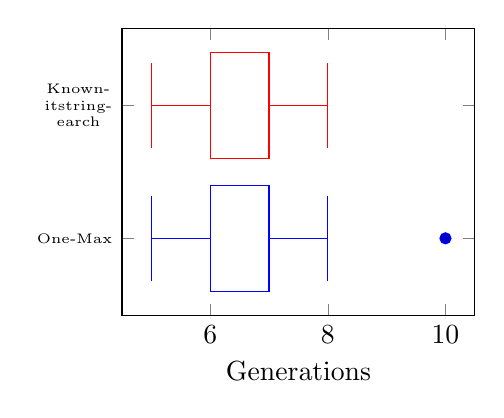
\begin{tikzpicture}
\begin{axis}
[
width=\textwidth/2,
ytick={1,2},
yticklabels={
    One-Max,
    Known-\\itstring-\\earch
},
yticklabel style={align=center,font=\tiny},
xlabel=Generations
]
\addplot+[boxplot]
table[row sep=\\, y index=0] {
% OneMax
data\\
7\\ 6\\ 6\\ 6\\ 7\\ 7\\ 5\\ 7\\ 7\\ 7\\ 8\\ 6\\ 6\\ 7\\ 7\\ 5\\ 7\\ 6\\ 7\\ 6\\ 7\\ 7\\ 7\\ 7\\ 7\\ 7\\ 7\\ 7\\ 7\\ 7\\ 7\\ 7\\ 7\\ 7\\ 7\\ 6\\ 7\\ 6\\ 6\\ 10\\ 7\\ 6\\ 6\\ 7\\ 6\\ 6\\ 7\\ 6\\ 7\\ 6\\ 7\\ 6\\ 7\\ 5\\ 6\\ 7\\ 7\\ 6\\ 6\\ 7\\ 7\\ 6\\ 7\\ 7\\ 7\\ 8\\ 7\\ 7\\ 7\\ 6\\ 7\\ 7\\ 7\\ 6\\ 8\\ 6\\ 7\\ 8\\ 7\\ 6\\ 7\\ 7\\ 7\\ 7\\ 6\\ 6\\ 7\\ 6\\ 7\\ 6\\ 7\\ 7\\ 6\\ 7\\ 7\\ 8\\ 6\\ 7\\ 6\\ 6\\
};
\addplot+[boxplot]
table[row sep=\\, y index=0] {
% Known-Bitstring-Search
data\\
6\\ 6\\ 7\\ 7\\ 6\\ 7\\ 7\\ 7\\ 7\\ 6\\ 6\\ 7\\ 7\\ 7\\ 7\\ 7\\ 7\\ 7\\ 6\\ 6\\ 6\\ 6\\ 7\\ 6\\ 8\\ 6\\ 6\\ 7\\ 6\\ 7\\ 7\\ 7\\ 7\\ 7\\ 7\\ 7\\ 6\\ 7\\ 6\\ 7\\ 7\\ 7\\ 7\\ 7\\ 8\\ 7\\ 6\\ 6\\ 7\\ 7\\ 7\\ 7\\ 7\\ 7\\ 6\\ 6\\ 7\\ 7\\ 6\\ 6\\ 6\\ 6\\ 5\\ 7\\ 7\\ 7\\ 6\\ 7\\ 7\\ 6\\ 8\\ 7\\ 7\\ 6\\ 7\\ 7\\ 7\\ 6\\ 6\\ 7\\ 6\\ 6\\ 6\\ 6\\ 7\\ 7\\ 8\\ 7\\ 6\\ 7\\ 6\\ 7\\ 7\\ 8\\ 7\\ 6\\ 7\\ 7\\ 6\\ 6\\
};
\end{axis}
\end{tikzpicture}
}
\caption{Box plot measurements of efficiency of solver runs mesured in generations until termination. Less is better. Whiskers represent the maximum and minimum measurement, the boxes contain measurements in the two center quartiles, and the center line is the median. Outliers are plotted as points. All measurements are measured over 100 runs of the solver for each case.}
\end{figure}


%\begin{figure}[H]
%\centering
%\subfloat[a]{\fitnessplot{
% generation 0
\addplot+[
boxplot prepared={
median=0.5625,
upper quartile=0.62015625,
lower quartile=0.54390625,
upper whisker=0.7225,
lower whisker=0.4225
},
] coordinates {};
% generation 5
\addplot+[
boxplot prepared={
median=0.62015625,
upper quartile=0.64,
lower quartile=0.5672265625,
upper whisker=0.70140625,
lower whisker=0.47265625
},
] coordinates {};
% generation 10
\addplot+[
boxplot prepared={
median=0.64,
upper quartile=0.70140625,
lower quartile=0.62015625,
upper whisker=0.74390625,
lower whisker=0.49
},
] coordinates {};
% generation 15
\addplot+[
boxplot prepared={
median=0.680625,
upper quartile=0.70140625,
lower quartile=0.64,
upper whisker=0.765625,
lower whisker=0.49
},
] coordinates {};
% generation 20
\addplot+[
boxplot prepared={
median=0.66015625,
upper quartile=0.70140625,
lower quartile=0.66015625,
upper whisker=0.765625,
lower whisker=0.58140625
},
] coordinates {};
% generation 25
\addplot+[
boxplot prepared={
median=0.680625,
upper quartile=0.70140625,
lower quartile=0.66015625,
upper whisker=0.765625,
lower whisker=0.600625
},
] coordinates {};
% generation 30
\addplot+[
boxplot prepared={
median=0.680625,
upper quartile=0.7225,
lower quartile=0.66015625,
upper whisker=0.78765625,
lower whisker=0.600625
},
] coordinates {};
% generation 35
\addplot+[
boxplot prepared={
median=0.680625,
upper quartile=0.7172265625,
lower quartile=0.66015625,
upper whisker=0.78765625,
lower whisker=0.58140625
},
] coordinates {};
% generation 40
\addplot+[
boxplot prepared={
median=0.70140625,
upper quartile=0.7225,
lower quartile=0.64,
upper whisker=0.78765625,
lower whisker=0.600625
},
] coordinates {};
% generation 45
\addplot+[
boxplot prepared={
median=0.70140625,
upper quartile=0.7225,
lower quartile=0.66015625,
upper whisker=0.78765625,
lower whisker=0.54390625
},
] coordinates {};
% generation 50
\addplot+[
boxplot prepared={
median=0.7225,
upper quartile=0.74390625,
lower quartile=0.680625,
upper whisker=0.92640625,
lower whisker=0.58140625
},
] coordinates {};
% generation 55
\addplot+[
boxplot prepared={
median=0.74390625,
upper quartile=0.765625,
lower quartile=0.7225,
upper whisker=0.92640625,
lower whisker=0.62015625
},
] coordinates {};
% generation 60
\addplot+[
boxplot prepared={
median=0.765625,
upper quartile=0.78765625,
lower quartile=0.74390625,
upper whisker=0.950625,
lower whisker=0.64
},
] coordinates {};
% generation 65
\addplot+[
boxplot prepared={
median=0.765625,
upper quartile=0.81,
lower quartile=0.74390625,
upper whisker=0.92640625,
lower whisker=0.64
},
] coordinates {};
% generation 70
\addplot+[
boxplot prepared={
median=0.83265625,
upper quartile=0.855625,
lower quartile=0.765625,
upper whisker=0.950625,
lower whisker=0.64
},
] coordinates {};
% generation 75
\addplot+[
boxplot prepared={
median=0.81,
upper quartile=0.855625,
lower quartile=0.78765625,
upper whisker=0.950625,
lower whisker=0.7225
},
] coordinates {};
% generation 80
\addplot+[
boxplot prepared={
median=0.83265625,
upper quartile=0.855625,
lower quartile=0.78765625,
upper whisker=0.950625,
lower whisker=0.70140625
},
] coordinates {};
% generation 85
\addplot+[
boxplot prepared={
median=0.83265625,
upper quartile=0.9025,
lower quartile=0.81,
upper whisker=0.97515625,
lower whisker=0.70140625
},
] coordinates {};
% generation 89
\addplot+[
boxplot prepared={
median=0.83265625,
upper quartile=0.901443390859,
lower quartile=0.789208692474,
upper whisker=1.0,
lower whisker=0.70140625
},
] coordinates {};
}
}
%\subfloat[b]{\fitnessplot{
% generation 0
\addplot+[
boxplot prepared={
median=0.5625,
upper quartile=0.600625,
lower quartile=0.525625,
upper whisker=0.70140625,
lower whisker=0.36
},
] coordinates {};
% generation 5
\addplot+[
boxplot prepared={
median=0.58140625,
upper quartile=0.64,
lower quartile=0.54390625,
upper whisker=0.7225,
lower whisker=0.455625
},
] coordinates {};
% generation 10
\addplot+[
boxplot prepared={
median=0.62015625,
upper quartile=0.6551171875,
lower quartile=0.5625,
upper whisker=0.765625,
lower whisker=0.49
},
] coordinates {};
% generation 15
\addplot+[
boxplot prepared={
median=0.66015625,
upper quartile=0.70140625,
lower quartile=0.62015625,
upper whisker=0.78765625,
lower whisker=0.50765625
},
] coordinates {};
% generation 20
\addplot+[
boxplot prepared={
median=0.680625,
upper quartile=0.7385546875,
lower quartile=0.64,
upper whisker=0.87890625,
lower whisker=0.54390625
},
] coordinates {};
% generation 25
\addplot+[
boxplot prepared={
median=0.70140625,
upper quartile=0.74390625,
lower quartile=0.66015625,
upper whisker=0.92640625,
lower whisker=0.50765625
},
] coordinates {};
% generation 30
\addplot+[
boxplot prepared={
median=0.70140625,
upper quartile=0.74390625,
lower quartile=0.66015625,
upper whisker=0.855625,
lower whisker=0.5625
},
] coordinates {};
% generation 35
\addplot+[
boxplot prepared={
median=0.7225,
upper quartile=0.765625,
lower quartile=0.680625,
upper whisker=0.855625,
lower whisker=0.58140625
},
] coordinates {};
% generation 40
\addplot+[
boxplot prepared={
median=0.74390625,
upper quartile=0.81,
lower quartile=0.7225,
upper whisker=0.87890625,
lower whisker=0.62015625
},
] coordinates {};
% generation 45
\addplot+[
boxplot prepared={
median=0.765625,
upper quartile=0.81,
lower quartile=0.7225,
upper whisker=0.9025,
lower whisker=0.64
},
] coordinates {};
% generation 50
\addplot+[
boxplot prepared={
median=0.78765625,
upper quartile=0.83265625,
lower quartile=0.765625,
upper whisker=0.9025,
lower whisker=0.66015625
},
] coordinates {};
% generation 55
\addplot+[
boxplot prepared={
median=0.81,
upper quartile=0.83265625,
lower quartile=0.765625,
upper whisker=0.9025,
lower whisker=0.680625
},
] coordinates {};
% generation 60
\addplot+[
boxplot prepared={
median=0.81,
upper quartile=0.83265625,
lower quartile=0.78765625,
upper whisker=0.9025,
lower whisker=0.680625
},
] coordinates {};
% generation 65
\addplot+[
boxplot prepared={
median=0.83265625,
upper quartile=0.855625,
lower quartile=0.78765625,
upper whisker=0.92640625,
lower whisker=0.70140625
},
] coordinates {};
% generation 70
\addplot+[
boxplot prepared={
median=0.83265625,
upper quartile=0.8730859375,
lower quartile=0.78765625,
upper whisker=0.950625,
lower whisker=0.70140625
},
] coordinates {};
% generation 71
\addplot+[
boxplot prepared={
median=0.83265625,
upper quartile=0.884112563993,
lower quartile=0.781562436007,
upper whisker=1.0,
lower whisker=0.70140625
},
] coordinates {};
}
}
%\qquad
%\subfloat[c]{\fitnessplot{
% generation 0
\addplot+[
boxplot prepared={
median=0.5625,
upper quartile=0.600625,
lower quartile=0.525625,
upper whisker=0.74390625,
lower whisker=0.4225
},
] coordinates {};
% generation 5
\addplot+[
boxplot prepared={
median=0.58140625,
upper quartile=0.64,
lower quartile=0.54390625,
upper whisker=0.74390625,
lower whisker=0.455625
},
] coordinates {};
% generation 10
\addplot+[
boxplot prepared={
median=0.62015625,
upper quartile=0.66015625,
lower quartile=0.58140625,
upper whisker=0.74390625,
lower whisker=0.50765625
},
] coordinates {};
% generation 15
\addplot+[
boxplot prepared={
median=0.66015625,
upper quartile=0.66015625,
lower quartile=0.66015625,
upper whisker=0.74390625,
lower whisker=0.50765625
},
] coordinates {};
% generation 20
\addplot+[
boxplot prepared={
median=0.66015625,
upper quartile=0.66015625,
lower quartile=0.66015625,
upper whisker=0.74390625,
lower whisker=0.525625
},
] coordinates {};
% generation 25
\addplot+[
boxplot prepared={
median=0.66015625,
upper quartile=0.66015625,
lower quartile=0.66015625,
upper whisker=0.74390625,
lower whisker=0.5625
},
] coordinates {};
% generation 30
\addplot+[
boxplot prepared={
median=0.66015625,
upper quartile=0.66015625,
lower quartile=0.66015625,
upper whisker=0.74390625,
lower whisker=0.5625
},
] coordinates {};
% generation 35
\addplot+[
boxplot prepared={
median=0.66015625,
upper quartile=0.66015625,
lower quartile=0.66015625,
upper whisker=0.74390625,
lower whisker=0.66015625
},
] coordinates {};
% generation 40
\addplot+[
boxplot prepared={
median=0.66015625,
upper quartile=0.66015625,
lower quartile=0.66015625,
upper whisker=0.74390625,
lower whisker=0.66015625
},
] coordinates {};
% generation 45
\addplot+[
boxplot prepared={
median=0.66015625,
upper quartile=0.70140625,
lower quartile=0.66015625,
upper whisker=0.74390625,
lower whisker=0.66015625
},
] coordinates {};
% generation 50
\addplot+[
boxplot prepared={
median=0.66015625,
upper quartile=0.70140625,
lower quartile=0.66015625,
upper whisker=0.74390625,
lower whisker=0.66015625
},
] coordinates {};
% generation 55
\addplot+[
boxplot prepared={
median=0.66015625,
upper quartile=0.70140625,
lower quartile=0.66015625,
upper whisker=0.74390625,
lower whisker=0.66015625
},
] coordinates {};
% generation 60
\addplot+[
boxplot prepared={
median=0.68078125,
upper quartile=0.70140625,
lower quartile=0.66015625,
upper whisker=0.74390625,
lower whisker=0.66015625
},
] coordinates {};
% generation 65
\addplot+[
boxplot prepared={
median=0.70140625,
upper quartile=0.70140625,
lower quartile=0.66015625,
upper whisker=0.74390625,
lower whisker=0.66015625
},
] coordinates {};
% generation 70
\addplot+[
boxplot prepared={
median=0.70140625,
upper quartile=0.70140625,
lower quartile=0.66015625,
upper whisker=0.74390625,
lower whisker=0.66015625
},
] coordinates {};
% generation 75
\addplot+[
boxplot prepared={
median=0.70140625,
upper quartile=0.74390625,
lower quartile=0.66015625,
upper whisker=0.74390625,
lower whisker=0.66015625
},
] coordinates {};
% generation 80
\addplot+[
boxplot prepared={
median=0.70140625,
upper quartile=0.74390625,
lower quartile=0.70140625,
upper whisker=0.74390625,
lower whisker=0.66015625
},
] coordinates {};
% generation 85
\addplot+[
boxplot prepared={
median=0.70140625,
upper quartile=0.74390625,
lower quartile=0.70140625,
upper whisker=0.74390625,
lower whisker=0.66015625
},
] coordinates {};
% generation 90
\addplot+[
boxplot prepared={
median=0.70140625,
upper quartile=0.74390625,
lower quartile=0.70140625,
upper whisker=0.74390625,
lower whisker=0.66015625
},
] coordinates {};
% generation 95
\addplot+[
boxplot prepared={
median=0.74390625,
upper quartile=0.74390625,
lower quartile=0.70140625,
upper whisker=0.74390625,
lower whisker=0.66015625
},
] coordinates {};
% generation 100
\addplot+[
boxplot prepared={
median=0.74390625,
upper quartile=0.74390625,
lower quartile=0.70140625,
upper whisker=0.74390625,
lower whisker=0.66015625
},
] coordinates {};
}
}
%\subfloat[d]{\fitnessplot{
% generation 0
\addplot+[
boxplot prepared={
median=0.5625,
upper quartile=0.62015625,
lower quartile=0.525625,
upper whisker=0.70140625,
lower whisker=0.43890625
},
] coordinates {};
% generation 5
\addplot+[
boxplot prepared={
median=0.5625,
upper quartile=0.600625,
lower quartile=0.525625,
upper whisker=0.74390625,
lower whisker=0.455625
},
] coordinates {};
% generation 10
\addplot+[
boxplot prepared={
median=0.5625,
upper quartile=0.600625,
lower quartile=0.525625,
upper whisker=0.680625,
lower whisker=0.455625
},
] coordinates {};
% generation 15
\addplot+[
boxplot prepared={
median=0.5625,
upper quartile=0.600625,
lower quartile=0.525625,
upper whisker=0.7225,
lower whisker=0.4225
},
] coordinates {};
% generation 20
\addplot+[
boxplot prepared={
median=0.54390625,
upper quartile=0.600625,
lower quartile=0.525625,
upper whisker=0.74390625,
lower whisker=0.37515625
},
] coordinates {};
% generation 25
\addplot+[
boxplot prepared={
median=0.5625,
upper quartile=0.600625,
lower quartile=0.50765625,
upper whisker=0.70140625,
lower whisker=0.40640625
},
] coordinates {};
% generation 30
\addplot+[
boxplot prepared={
median=0.5625,
upper quartile=0.600625,
lower quartile=0.525625,
upper whisker=0.74390625,
lower whisker=0.4225
},
] coordinates {};
% generation 35
\addplot+[
boxplot prepared={
median=0.5625,
upper quartile=0.600625,
lower quartile=0.525625,
upper whisker=0.74390625,
lower whisker=0.43890625
},
] coordinates {};
% generation 40
\addplot+[
boxplot prepared={
median=0.5625,
upper quartile=0.600625,
lower quartile=0.50765625,
upper whisker=0.7225,
lower whisker=0.4225
},
] coordinates {};
% generation 45
\addplot+[
boxplot prepared={
median=0.5625,
upper quartile=0.600625,
lower quartile=0.5121484375,
upper whisker=0.74390625,
lower whisker=0.4225
},
] coordinates {};
% generation 50
\addplot+[
boxplot prepared={
median=0.5625,
upper quartile=0.600625,
lower quartile=0.525625,
upper whisker=0.680625,
lower whisker=0.390625
},
] coordinates {};
% generation 55
\addplot+[
boxplot prepared={
median=0.54390625,
upper quartile=0.600625,
lower quartile=0.50765625,
upper whisker=0.74390625,
lower whisker=0.43890625
},
] coordinates {};
% generation 60
\addplot+[
boxplot prepared={
median=0.5625,
upper quartile=0.6152734375,
lower quartile=0.525625,
upper whisker=0.78765625,
lower whisker=0.455625
},
] coordinates {};
% generation 65
\addplot+[
boxplot prepared={
median=0.5625,
upper quartile=0.600625,
lower quartile=0.525625,
upper whisker=0.78765625,
lower whisker=0.40640625
},
] coordinates {};
% generation 70
\addplot+[
boxplot prepared={
median=0.5625,
upper quartile=0.62015625,
lower quartile=0.525625,
upper whisker=0.765625,
lower whisker=0.455625
},
] coordinates {};
% generation 75
\addplot+[
boxplot prepared={
median=0.58140625,
upper quartile=0.600625,
lower quartile=0.525625,
upper whisker=0.74390625,
lower whisker=0.40640625
},
] coordinates {};
% generation 80
\addplot+[
boxplot prepared={
median=0.553203125,
upper quartile=0.58140625,
lower quartile=0.50765625,
upper whisker=0.7225,
lower whisker=0.40640625
},
] coordinates {};
% generation 85
\addplot+[
boxplot prepared={
median=0.54390625,
upper quartile=0.5958203125,
lower quartile=0.525625,
upper whisker=0.78765625,
lower whisker=0.4225
},
] coordinates {};
% generation 90
\addplot+[
boxplot prepared={
median=0.5625,
upper quartile=0.600625,
lower quartile=0.525625,
upper whisker=0.70140625,
lower whisker=0.455625
},
] coordinates {};
% generation 95
\addplot+[
boxplot prepared={
median=0.5625,
upper quartile=0.600625,
lower quartile=0.525625,
upper whisker=0.74390625,
lower whisker=0.43890625
},
] coordinates {};
% generation 100
\addplot+[
boxplot prepared={
median=0.5625,
upper quartile=0.62015625,
lower quartile=0.525625,
upper whisker=0.74390625,
lower whisker=0.43890625
},
] coordinates {};
}
}
%\end{figure}

\end{document}
